\documentclass[12pt,a4paper]{article}

\usepackage{lmtstyle}
\usepackage[BCOR1cm]{typearea}
\usepackage[american]{babel}
\usepackage{tocbibind}
\usepackage{parskip}
\usepackage[latin1]{inputenc}
\usepackage{a4wide}
\usepackage{makeidx}
\usepackage{url}
\usepackage{doc}
\usepackage{graphicx}
\usepackage{color}
\usepackage{amsmath}
\usepackage{amsfonts}
\usepackage{amssymb}
\usepackage{amsthm}
\usepackage{enumerate}
\usepackage{tikz}
\usepackage{wrapfig}

\usetikzlibrary{arrows,calc,patterns,angles,quotes}
\usepackage{caption}
\captionsetup[table]{position=bottom} 
\usepackage[ruled,lined]{algorithm2e}
\DontPrintSemicolon

\newcommand{\norm}[1]{\left\lVert#1\right\rVert}
\newcommand{\expec}[1]{\mathbb{E}\left[#1\right]}
\newcommand{\G}{\mathcal{G}}
\renewcommand{\P}{\mathbb{P}}
\renewcommand{\d}{\text{d}}
\newcommand{\trarrow}[1]{\xrightarrow{\text{#1}}}
\newtheoremstyle{def}
  {12pt}   % ABOVESPACE
  {6pt}   % BELOWSPACE
  {\normalfont}  % BODYFONT
  {0pt}       % INDENT (empty value is the same as 0pt)
  {\bfseries} % HEADFONT
  {.}         % HEADPUNCT
  {5pt plus 1pt minus 1pt} % HEADSPACE
  {}          % CUSTOM-HEAD-SPEC

\theoremstyle{def}
\newtheorem{theorem}{Theorem}[section]
\theoremstyle{def}
\newtheorem{lemma}[theorem]{Lemma}
\theoremstyle{def}
\newtheorem{assumption}[theorem]{Assumption}
\newtheorem*{remark}{Remark}
\newtheorem*{remarks}{Remarks}
\theoremstyle{def}
\newtheorem{definition}[theorem]{Definition}

\graphicspath{{figures/}}

\global\newcommand{\note}[1]{{\color{red}(#1)}}

\title{Sequential Monte Carlo for time-dependent Bayesian Inverse Problems}
\author{Matthieu Bult�}
\advisor{M.Sc. Jonas Latz}
\supervisor{Prof. Dr. Elisabeth Ullmann}
\dateend{15. June 2018}

\begin{document}

\makemtgtitle
 
\thispagestyle{plain}
\pagenumbering{gobble}
\vspace*{1cm}
With my signature below, I assert that the work in this thesis has been composed by myself independently and no source materials or aids other than those mentioned in the thesis have been used.

\vspace{2cm}

\hspace{1cm}
\begin{tabular}{ccc}
  \vspace{-0.3cm}M\"unchen, \today 	&\hspace{4cm} 		& \\
  \rule{4.5cm}{0.4pt}					&					&\rule{4.5cm}{0.4pt}\\
  Place, Date							&					& Signature			
\end{tabular}           		

\vspace{4cm}
This work is licensed under the Creative Commons Attribution 3.0 Germany License. To view a copy of the license, visit http://creativecommons.org/licenses/by/3.0/de\\

Or\\

Send a letter to Creative Commons, 171 Second Street, Suite 300, San Francisco, California 94105, USA.
%%% Local Variables:
%%% mode: latex
%%% TeX-master: "LMT_Thesis"
%%% End:


\numberwithin{equation}{section}
\pagenumbering{roman}
\thispagestyle{plain}

\section*{Abstract}

%%% Local Variables:
%%% mode: latex
%%% TeX-master: "Thesis"
%%% End:

\tableofcontents

\section{Introduction}
\pagenumbering{arabic}
\setcounter{page}{1}
\thispagestyle{empty}

The study of complex systems is often done through mathematical modelling, allowing the simulation, analysis and prediction of their behaviour. These mathematical models require input parameters, for which only limited or no information is known. Finding these parameters from measurements of the system is called the \textit{inverse problem}. Since measurements are often noisy or sparse, and the mathematical models can be complex and expensive to evaluate, developing sound and efficient mathematical frameworks to treat the inverse problem is a complicated task.

Two prominent classes of methods for attempting to address this problem are the \textit{maximum likelihood} methods and the \textit{Bayesian} methods. In maximum likelihood methods, the solution of the inverse problem is given as the maximizer of the likelihood of the observed data. In Bayesian methods, the system is re-modeled probabilistically with random variables. This solution is given as a marginalization of the model by the observed data using Bayes' formula, as first developed by Laplace \cite{laplace1820theorie}. A theoretical and practical comparison of the two methods is given by Kaipio and Somersalo \cite{kaipio2006statistical}, including a broad introduction to solving inverse problems found in science and engineering. 

The Bayesian approach is a very general modelling and inference framework allowing to address very different kinds of statistical problems. The work by Gelman et al. \cite{gelman} gives a broad introduction to the field of \textit{Bayesian data analysis}. Based on the framework presented by Stuart \cite{stuart_2010} on Bayesian methods for inverse problems, we focus on the application of Bayesian inference to time-dependent inverse problems, called \textit{Bayesian filtering}. We will demonstrate that under weak model assumptions, the solution can be shown to be \textit{well-posed}, using a definition of well-posedness similar to Hadamard's \cite{hadamard}.

Very often, the solution of an inverse problem given in the Bayesian framework does not admit any analytical solution. Since one is interested in obtaining summarized statistics about the solution of the inverse problem, such as mean and variance, numerical approximations will involve computing integrals over the parameter space. Since volumes grow exponentially with the number of dimensions, classical methods of numerical integration cannot be used for high-dimensional problems. This phenomenon is called the \textit{curse of dimensionality}.

Fortunately, other numerical approximations were developed that do not suffer from the curse of dimensionality. Typically, such approximations work by generating pseudo-random values distributed according to the posterior distribution and use them to approximate the hard integral. Some variation of the law of large numbers will then provide dimensionality-free error bounds, making these methods suited for high-dimensional problems. A common class of algorithms falling in this category are the \textit{Markov Chain Monte Carlo} (MCMC) methods, presented by Metropolis et al. \cite{metropolis1953equation} for a specific class of problems, and later extended to the general case by Hastings \cite{hastings1970monte}. While having dimensionality-free error bounds, MCMC algorithms often need a lot of knowledge and tunning to properly operate. A simpler method to operate is \textit{importance sampling} (IS) \cite{Robert}, where the sampling is done by choosing an auxiliary distribution that is similar to the target distribution, but from which direct sampling is easier. The discrepancy between the generated samples and a sample generated from the posterior distribution is then corrected by assigning correction weights to the values of the sample. However, choosing an auxiliary distribution that is close to the target distribution is not always possible, and failling to do so results in a poor estimation of the posterior distribution.

\textit{Sequential Monte Carlo} (SMC) \cite{del_moral_2006} is a method merging ideas of MCMC and IS samplers in an attempt to solve major problems found in these other two methods. This sampler was created to approximate sequences of distributions, such as those found in data assimilation problems. However, it can also be used on an artificial sequence of distributions to interpolate between a simple initial auxiliary distribution and the true posterior. This is done by Beskos et al. \cite{beskos2015sequential} for approximating the solution of a Bayesian inverse problem associated to elliptic PDEs. By drawing parallels to particle physics, Del Moral \cite{del2013mean, del2004feynman} provides convergence results of the algorithm that will be presented in this thesis.

In their work, Allmaras et al. \cite{bayes-tutorial} give a case study-based introduction to the whole process of Bayesian techniques for solving inverse problems. This thesis will follow a similar approach, by structuring itself around a simple time-dependent Bayesian filtering problem. The system studied is the simple pendulum, an idealized model for a pendulum in which the mass of the pendulum and the air friction are ignored. It can be described by a second-order, non-linear differential equation with a parameter representing the \textit{gravitational acceleration}. We will describe the model of the pendulum, together with the inversion task of estimating the gravitational acceleration from a set of measurements taken in an experiment. 


The rest of the thesis is structured as follows. In Section 2, we describe time-dependent inverse problems and Bayesian filtering. Moreover, we show how to formulate the pendulum problem in the Bayesian framework. In Section 3, we present the construction of the SMC algorithm and show the parallels to IS and MCMC. We also present a proof of convergence of the algorithm and discuss possible extensions. We conclude the section by computing and comparing numerical solutions to the pendulum problem. Finally, Section 4 discusses other application areas and current research on SMC algorithms.

%%% Local Variables:
%%% mode: latex
%%% TeX-master: "Thesis"
%%% End:

\section{Bayesian Filtering}

This section introduces and describes the Bayesian approach for solving inverse problems, laying out the theoretical foundations of the taken approach. In Section 2.1 we present the class of problems we will be considering in this thesis: finite-dimensional inverse and filtering problems. In Section 2.2 we present a filtering problem based on a simple dynamical system estimation problem which will be used to illustrate concepts presented throughout the thesis. In Section 2.3 we define desired characteristics of solutions to inverse problems. We mention the challenges encountered by the classical optimization approach for solving inverse problems in practical situations. We then present the Bayesian framework, and show how it uses prior information about the structure of the problem to construct a solution to the inverse and filtering problems. In Section 2.4 we prove well-posedness of this constructed solution under some light assumptions about the model. Finally, Section 2.5 illustrates Bayesian modelling by describing the process of constructing a probabilistic model for the pendulum problem, and show that the problem is well-posed and thus admits a stable solution.

\subsection{Set-Up}

We study parametrized models for which the value of the \textit{parameter} $u \in X$ is unknown or uncertain. To model the behaviour of the system, we introduce a \textit{forward response operator} $\mathcal{G} : X \rightarrow Y$ mapping values of the \textit{parameter space} to the \textit{data space}, assuming both spaces to be finite-dimensional vector spaces.

We consider a real system described by $\mathcal{G}$ and the true parameter $u^* \in X$, and assume that \textit{observations} $y^{obs} \in Y$ of the system are available from measurements. The data $y$ is then the image of the true parameter under the mapping $\mathcal{G}$. We obtain the following model

\begin{equation}\label{inverse-formula}
  y^{obs} = \G(u^*),
\end{equation}

where the equality is not exact due to uncertainties. Our initial question then becomes: \textit{to which extent can we find the inverse of the data $y^{obs}$ under the forward response operator $\G$?} Answering this question is known as the \textit{inverse problem}.

In this thesis, we are interested in solving the inverse problem by incrementally building up knowledge about the unknown parameter $u^*$. To do this, we decompose the data and consider a growing sequence of observations made available for analysis. The advantages of this approach are twofold. Firstly, it allows to perform inference on running dynamical systems and update our knowledge as more measurements become available. Secondly, it can also be used in situations where all the data is available to transform one large problem in a sequence of smaller problems that can hopefully be solved more efficiently.

In this sequential formulation, the data $y$ is decomposed in a finite sequence of observations $y^{obs} = (y^{obs}_1, \ldots, y^{obs}_T)^\top$. We also decompose the forward response operator $\G$ in a sequence of operators $\G_1, \ldots, \G_T$ such that

\begin{equation*}
  y^{obs}_t = \G_t(u^*).
\end{equation*}

This allows us to reformulate the question from above as \textit{How can we use new observations to update our knowledge about $u^*$?} Answering this new question is called the \textit{filtering problem}. This thesis will focus on solving inverse and filtering problems.

One situation where this decomposition can naturally be used is when the system is described by an initial value problem of the form

\begin{equation}
  \begin{aligned}
    x'(t) &= f(x(t); u)\\
    x(0) &= x_0,
  \end{aligned}
\end{equation}  

where $u \in X$ is the parameter of the model, and the solution $x(t; u)$ is assumed to exist for every time $t \geq 0$. The sequence of observations then correspond to measurements at times  $0 \leq t_1 < \ldots < t_T$. We further define two additional kinds of operators: \textit{solution} and \textit{observational} operators. The solution operator $G$ maps elements of the parameter space to the solution of the associated initial value problem by $G(u) = x(\cdot, u)$. Observational operators $\mathcal{O}_i$ then map this solution to the respective observation, here we can define for each time $t_i$ the observational operator $\mathcal{O}_i(x(\cdot, u)) = x(t_i, u)$. The forward response operators can then be written as the composition of these two operators $\G_i = \mathcal{O}_i \circ G$. We provide an example of the modelling of a inverse problem in the next section.

\subsection{Pendulum problem}

We now introduce a filtering problem that will guide the rest of the thesis. Using a pendulum, we would like to estimate the value of the Earth's gravitational acceleration. We start by modelling the behaviour of the pendulum using a differential equation parametrized by the gravitational acceleration $g$.

We choose the \textit{simple pendulum model}, a simplified mathematical model that ignores the mass of the string of the pendulum and ignores the forces of friction acting on the hanging mass. It also assumes that the movement of the pendulum only happens in two dimensions. This simplification allows us to model the state of the pendulum with a single value $x(t)$ representing the angle of the pendulum to the resting point, described by the following second ordinary order differential equation.

\begin{equation}\label{pendulum-ode}
  \begin{aligned}
  x''(t) &= -\frac{g}{l}\sin(x(t))\\
  x'(0) &= x'_0\\
  x(0) &= x_0.
  \end{aligned}
\end{equation}

In this model, $g$ is the Earth's gravitational acceleration and $l$ is the length of the string holding the hanging mass. A representation of this model is given in Figure \ref{pendulum-fig}.

We then run an experiment in which the pendulum is let go from an initial angle of $x_0 = 5\pi/180\ (5^\circ)$ and no initial velocity $x'_0 = 0$. Using a stopwatch, we collect $T=11$ time measurements at which the pendulum was aligned with the vertical axis, corresponding to a null angle of the pendulum.

\begin{figure}
  \centering
  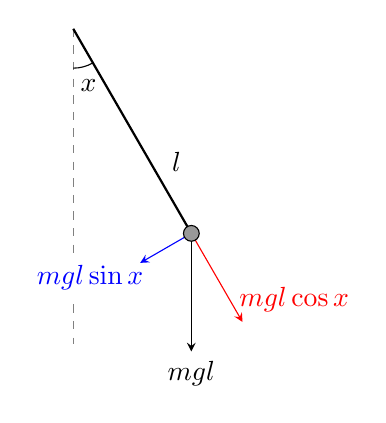
\begin{tikzpicture}
    % save length of g-vector and theta to macros
    \pgfmathsetmacro{\Gvec}{1.5}
    \pgfmathsetmacro{\myAngle}{30}
    % calculate lengths of vector components
    \pgfmathsetmacro{\Gcos}{\Gvec*cos(\myAngle)}
    \pgfmathsetmacro{\Gsin}{\Gvec*sin(\myAngle)}

    \coordinate (centro) at (0,0);
    \draw[dashed,gray,-] (centro) -- ++ (0,-2.9) node (mary) [black,below]{$ $};
    \draw[dashed,gray,-] (0,-3.5) -- ++ (0,-0.5);
    \draw[thick] (centro) -- ++(270+\myAngle:3) coordinate (bob)
      node[near end,above right] {$l$};
    \pic [draw, -, "$x$", angle eccentricity=1.5] {angle = mary--centro--bob};
    \draw [red,-stealth] (bob) -- ($(bob)!-\Gcos cm!(centro)$)
      coordinate (gcos)
      node[near end, right] {$mgl\cos x$};
    \draw [blue,-stealth] (bob) -- ($(bob)!\Gsin cm!90:(centro)$)
      coordinate (gsin)
      node[near end,below left] {$mgl\sin x$};
    \draw [-stealth] (bob) -- ++(0,-\Gvec)
      coordinate (g)
      node[below] {$mgl$};
    \filldraw [fill=black!40,draw=black] (bob) circle[radius=0.1];
\end{tikzpicture}


%%% Local Variables:
%%% mode: latex
%%% TeX-master: "Thesis"
%%% End:

  \caption{Pendulum model and forces applied to the mass, the vertical vector represents the gravitational force and the red and blue vectors represent the same force decomposed into its components, parallel and perpendicular to the motion of the pendulum. The dashed line represents the $0$ angle at which measurements are taken.}
  \label{pendulum-fig}
\end{figure}

\subsection{Bayesian filtering}

The previous sections defined the inverse and filtering problems. Before starting to discuss solutions to these problems, we present the concept of \textit{well-posedness} first given by Hadamard in \cite{hadamard} for describing properties of models of physical phenomena.

\begin{definition} A problem is said to be \textit{well-posed} if it satisfies the following conditions:
  \begin{enumerate}
  \item{a solution exists,}
  \item{the solution is unique,}
  \item{the solution changes continuously with respect to the data.}
  \end{enumerate}

  A problem failing to satisfy these conditions is said to be \textit{ill-posed}. In the context of inverse problems, the third property states that small perturbations in the data should result in proportionally small perturbations in the solution $u$ of the inverse problem. 
\end{definition}

A possible way to solve inverse problems is to try to find a value $\hat u \in X$ that solves the inverse problem \textit{as well as possible}. This is done by replacing the inverse problem by the following non-linear least squares problem

\begin{equation*}
  \hat u = \underset{u \in X}{\text{argmin}} \frac12\norm{ y^{obs} - \G(u) }_Y^2.
\end{equation*}

However, finding a global minimum in the presence of noise is often a difficult task since it might not exist, or the minimized function might admit multiple local minima. Solving the inverse problem by minimization is thus an ill-posed problem. While some of these difficulties can be addressed by \textit{regularization}, two issues remain unresolved. Firstly, regularization and the choice of the minimized norm are \textit{ad hoc} decisions that are not part of the modelling process. Secondly, assuming that the optimization algorithm does provide an estimate $\hat u$, this point estimate does not contain information about the quality, nor \textit{uncertainty}, of this estimation. For these reasons, we chose to study a different approach for solving inverse problems: the Bayesian framework.

In the Bayesian framework, the model is treated as an encoding of the relation between the knowns and the unknowns of the system, as opposed to being treated as an equation that has to be inverted. In this encoding, we represent every variable using \textit{random variables} and refine the model to include every available information of the system. This allows us to rewrite the standard inverse problem as follows

\begin{equation}\label{prob-inv}
  y = \G(u) + \eta.
\end{equation}

Here, the variable $y$ models the measurements of the system, and the observations $y^{obs}$ are treated as realizations of this random variable. Existing knowledge about the parameter prior to collecting the data is incorporated in the distribution of $u$, called the \textit{prior distribution} with measure $\mu_0$. The remaining variable $\eta$ is used to represent the uncertainty in $y$, such as measurement noise and modelling error. These uncertainties are often modelled using a mean-zero Gaussian distribution.

The coupling of these random variables given by (\ref{prob-inv}) allows us to answer a wide range of questions about the model through the use of conditioning. For instance, we can consider the probability density of the conditioned random variable $y|u$, called the \textit{likelihood function}. If $\rho$ denotes the density function of $\eta$, the likelihood function is

\begin{equation}\label{def-ell}
  \ell(y|u) := \rho(y - \G(u)).
\end{equation}

The observations are then realizations of the \textit{data-generating measure} with density $\ell(y|u^*)$, where $u^*$ is fix. Motivated by the wide use of the Gaussian distribution for error modelling, we assume throughout the thesis that the likelihood function can be written as

\begin{equation} \label{exponential-ell}
  \ell(y|u) = \exp(-\Phi(u;y)),
\end{equation}

where $\Phi$ is called a \textit{potential function}, or \textit{negative log-likelihood}. In the case where the uncertainty is modeled by a multivariate Gaussian distribution $\eta \sim \mathcal{N}(0, \Gamma)$, the potential function is given by

\begin{equation} \label{gaussian-potential}
  \Phi(u; y) = \norm{\Gamma^{-1/2}(y - \G(u))}_Y^2.
\end{equation}

When solving the inverse problem, we are interested in using observed data to update our prior believes about the model's parameter $u$. This question can be naturally translated into studying the conditional distribution of $u$ under the observation $y = y^{obs}$. The new knowledge about the parameter $u$ is then contained in the distribution of $u$ given $y$, called the \textit{posterior distribution} with measure $\mu^y$. Intuitively, \textit{Bayes' rule} can be used to find the posterior distribution in terms of the prior distribution and the likelihood.

Given a probability space $(\Omega, \mathcal{F}, \P)$, and two events $A, B \in \mathcal{F}$ with $\P(B) > 0$, Bayes' rule gives the distribution of the conditioned event by

\begin{equation*}
  \P(A|B) = \frac{\P(B|A)\P(A)}{\P(B)}.
\end{equation*}

An informal extension of this theorem to infinitesimal events gives the following relation for the posterior distribution 

\begin{equation}\label{bayes-rule}
  \d\mu^y(u) \propto \ell(y|u)\d\mu_0(u),
\end{equation}

where the $\propto$ symbol denotes proportionality up to a constant factor $Z_y$ only dependent on the data $y$, called the \textit{normalizing constant} or \textit{model evidence}, and given by

\begin{equation}
 Z_y = \int_X \ell(y|u)\d\mu_0(u).
\end{equation}

This framework for solving inverse problems can be used to express filtering problems, and thus also provide a solution to the latter. 

Extending the proposed formulation of inverse problems to filtering problems is done in an intuitive way. The use of a prior distribution to model existing knowledge about the model paramater remains unchanged. However, more structure has to be given to the uncertainty since it now requires a sequence of independent random variables $\eta_1, \ldots, \eta_T$ for each step of the filtering. This provides us with a sequence of potentials $\Phi_1, \ldots, \Phi_T$ and likelihoods $\ell_1, \ldots, \ell_T$, which in turn provide us with a sequence of partial solutions

\begin{equation*}
  \d\mu_t^y(u) \propto \ell_t(u|y_{1:t})\d\mu_0(u).
\end{equation*}

However, when no natural sequence of intermediate measures exists, we need to create this sequence artificially. One common way to create this sequence of artificial states is to consider an increasing subset of the observations for each of these measures. Given the forward response operator $\G : X \rightarrow Y^T$, we consider the sequence of potentials

\begin{equation}\label{phi-seq}
  \Phi_t(u; y) = \norm{y_{1:t} - \G(u)_{1:t}}_{Y^t}^2 = \sum_{i=1}^t\norm{y_i - \G_i(u)}_Y^2.
\end{equation}

This method has two main advantages. Firstly, it does not require to have all observations available at each step of the filtering, allowing to perform inference on a running experiment. Secondly, the sequence of posteriors acts as an interpolation between the prior and the posterior, as illustrated in the right panel of Figure \ref{uncertainty-posteriors} of page 15. This property will be shown to be central in the design of the numerical approximations presented later.

While the argument presented above provides the correct result, the extension of Bayes' rule from events to probability measures is not valid. Moreover, it is not clear which assumptions were made about the model to ensure existence the solutions, and more generally, well-posedness has not been discussed. We present a more rigorous proof and characterization of well-posed inverse problems in the following section.

\subsection{Well-posedness of Bayesian inverse problems}

In this section, we will focus on well-posedness of Bayesian inverse problems. However, as shown in the previous section, a filtering problem can be interpreted as a sequence of inverse problems defined by forward response operators and likelihoods $(\G_1, \ell_1), \ldots, (\G_T, \ell_T)$. A filtering problem is then said to be well-posed if every intermediate inverse problem is well-posed.


We start by stating the following assumptions proposed by Stuart \cite{stuart_2010}

\begin{assumption} \label{assumption-ll}
  The function $\Phi : X \times Y \rightarrow \mathbb{R}$ has the following properties.
  
  \begin{enumerate}
  \item For every $\epsilon > 0$ and $r > 0$ there is an $M \in \mathbb{R}$ such that, for all $u \in X$ and all $y \in Y$ with $\norm{y}_Y < r$,
    \begin{equation*}
      \Phi(u; y) \ge M - \epsilon\norm{u}_X^2.
    \end{equation*}
  \item For every $r > 0$ there is a $K > 0$ such that, for all $u \in X$ and $y \in Y$ with $\text{max}\{\norm{u}_X, \norm{y}_Y\} < r$,
    \begin{equation*}
      \Phi(u; y) \le K.
    \end{equation*}

  \item For every $r > 0$ there is a $L > 0$ such that, for all $u_1, u_2 \in X$ and $y \in Y$ with $\text{max}\{\norm{u_1}_X, \norm{u_2}_X, \norm{y}_Y\} < r$,

    \begin{equation*}
      |\Phi(u_1; y) - \Phi(u_2; y)| \le L\norm{u_1 - u_2}_X.
    \end{equation*}

  \item For every $\epsilon > 0$ and $r > 0$ there is a $C \in \mathbb{R}$ such that, for all $y_1, y_2 \in Y$ with $\text{max}\{\norm{y_1}_Y, \norm{y_2}_Y\} < r$, and for all $u \in X$,

    \begin{equation*}
      |\Phi(u; y_1) - \Phi(u; y_2)| \le \exp(\epsilon\norm{u}_X^2 + C)\norm{y_1 - y_2}_Y.
    \end{equation*}
  \end{enumerate}
\end{assumption}

These mild assumptions happen to be rather easy to fulfill for many practical problems. These assumptions provide us with upper and lower bounds on $\Phi$, as well as its Lipschitz continuity with respect to the data $y$ and the parameter $u$.  However, since potential functions are often of the form of (\ref{gaussian-potential}), we are interested in refining these assumptions to the shared structure of such problems.

\begin{assumption}\label{assumption-fw}
  The function $\G : X \rightarrow \mathbb{R}^N$ has the following properties.

  \begin{enumerate}
  \item For every $\epsilon > 0$ there is an $M \in \mathbb{R}$ such that for all $u \in X$,
    \begin{equation*}
      \norm{\G(u)}_\Gamma \le \exp(\epsilon \norm{u}_X^2 + M).
    \end{equation*}
  \item For every $r > 0$ there is a $K > 0$ such that, for all $u_1, u_2 \in X$ with $\text{max}\{\norm{u_1}_X, \norm{u_2}_X\} < r$,
    \begin{equation*}
      \norm{\G(u_1) - \G(u_2)}_\Gamma \le K\norm{u_1 - u_2}_X.
    \end{equation*}
  \end{enumerate}
\end{assumption}

We can naturally use these assumptions on the forward response operator $\G$ to derive properties of the potential function using the following lemma.

\begin{lemma} \label{fw-implies-ll}
  Assume that $\G  : X \rightarrow \mathbb{R}^N$ satisfies Assumption \ref{assumption-fw}. Then, for any covariance matrix $\Gamma$, the potential function given by (\ref{gaussian-potential}) satisfies Assumption \ref{assumption-ll} with $(Y, \norm{\cdot}_Y) = (\mathbb{R}^N, \norm{\cdot}_\Gamma)$.
\end{lemma}

\begin{proof}
  Let $\G : X \rightarrow \mathbb{R}^N$ be a forward operator satisfying Assumption \ref{assumption-fw}, $\Gamma$ be a covariance matrix and $\Phi$ be the potential function given by (\ref{gaussian-potential}), i.e. $\Phi(u; y) = \norm{y - \G(u)}_\Gamma^2$. We now prove $\Phi$ satisfies Assumptions \ref{assumption-ll}(1-4).

  1. Let $\epsilon > 0$ and $r > 0$, then for $M = 0$ and all $u \in X$, $y \in Y$ with $\norm{y}_Y < r$ we have by positivity of the norms $\norm{\cdot}_\Gamma$ and $\norm{\cdot}_X$
  \begin{equation*}
    \Phi(u; y) = \norm{y - \G(u)}_\Gamma^2 \ge 0 \ge 0 - \epsilon\norm{u}_X^2 = M - \epsilon\norm{u}_X^2.
  \end{equation*}

  2. Let $r > 0$, then from Assumption \ref{assumption-fw}(1) there is for $\epsilon = 1$ an $M \in \mathbb{R}$ such that $\norm{\G(u)}_\Gamma \le \exp(\norm{u}_X^2 + M)$ for every $u \in X$. Let $K = r^2 + \exp(2r^2 + 2M) > 0$, then for all $u \in X$ and $y \in Y$ with $\max{\norm{u}_X, \norm{y}_\Gamma} < r$ we have by
  \begin{equation*}
    \Phi(u; y) = \norm{y - \G(u)}_\Gamma^2 \le \norm{y}_\Gamma^2 + \norm{\G(u)}_\Gamma^2 \le \norm{y}_\Gamma^2 + \exp(\norm{u}_X^2 + M)^2 \le  K.
  \end{equation*}

  3. Let $r > 0$, from Assumption \ref{assumption-fw}(2) there is a $K > 0$ such that for every $u_1, u_2 \in X$ with $\max\{\norm{u_1}_X, \norm{u_2}_X\} < r$ we have $\norm{\G(u_1) - \G(u_2)}_\Gamma \le K\norm{u_1 - u_2}_X$. Let $L = 2rK^2$, for all $u_1, u_2 \in X$ and $y \in Y$ with $\max\{\norm{u_1}_X, \norm{u_2}_X,\norm{y}_\Gamma\} < r$ we obtain by definition of $L$ and reverse triangle inequality
  \begin{align*}
    |\Phi(u_1; y) - \Phi(u_2; y)|
    &= \left|\norm{y - \G(u_1)}_\Gamma^2 - \norm{y - \G(u_2)}_\Gamma^2\right|
    \le \norm{ (y - \G(u_1)) - (y - \G(u_2))}_\Gamma^2\\
    &= \norm{\G(u_1) - \G(u_2)}_\Gamma^2 \le K^2\norm{u_1 - u_2}_X^2 \le L\norm{u_1 - u_2}_X.
  \end{align*}

  4. Let $\epsilon > 0$, $r > 0$ and $y_1, y_2 \in Y$ with $\max\{\norm{y_1}_\Gamma, \norm{y_2}_\Gamma\} < r$ and $u \in X$ be arbitrary. Since $\Phi$ is continuously differentiable with respect to $y$, we obtain
  \begin{equation*}
    |\Phi(u; y_1) - \Phi(u; y_2)|
    \le \underset{\norm{y}_\Gamma \le r}{\sup}\norm{\nabla_y \Phi(u; y)}_\Gamma\norm{y_1 - y_2}_\Gamma.
  \end{equation*}
  Additionally, since $\nabla_y \Phi(u; y) = 2\langle y - \G(u), \cdot\rangle_\Gamma$ and making use of the Cauchy-Schwarz inequality, we have for any $y \in Y$
  \begin{align*}
    \norm{\nabla_y \Phi(u; y)}_\Gamma
    &= \underset{\norm{w}_\Gamma = 1}{\sup} |\nabla_y \Phi(u; y)[w]|
    = \underset{\norm{w}_\Gamma = 1}{\sup} 2|\langle y - \G(u), w\rangle_\Gamma|
    \\ &\le \underset{\norm{w}_\Gamma = 1}{\sup}2\norm{y - \G(u)}_\Gamma\norm{w}_\Gamma = 2\norm{y - \G(u)}_\Gamma.
  \end{align*}
  Furthermore, using Assumption \ref{assumption-fw}(2) there is an $M \in \mathbb{R}$ such that $\norm{G(u)}_\Gamma \le \exp(\epsilon \norm{u}_X^2 + M)$ for all $u \in X$, giving for any $y \in Y$ with $\norm{y}_\Gamma \le r$
  \begin{align*}
    \norm{y - \G(u)}_\Gamma
    &\le \norm{y}_\Gamma + \norm{\G(u)}_\Gamma
    \le r + \exp(\epsilon\norm{u}_X^2 + M)\\
    &= \exp(\epsilon\norm{u}_X^2 + M)(r \exp(-\epsilon\norm{u}_X - M) + 1)\\
    &\le \exp(\epsilon\norm{u}_X^2 + M)(r \exp(-M) + 1)\\
    &= \exp(\epsilon\norm{u}_X^2 + C),
  \end{align*}
  where $C = M + \log(r \exp(-M) + 1)$. All together, we obtain the desired bound
  \begin{equation*}
    |\Phi(u; y_1) - \Phi(u; y_2)| \le \exp(\epsilon \norm{u}_X^2 + C)\norm{y_1 - y_2}.
  \end{equation*}
\end{proof}

Using these assumptions, we can now proceed to provide a formal proof of Bayes' rule for continuous random variables and of equation (\ref{bayes-rule}), which we recall gives the following relation for the posterior distribution

\begin{equation*}
  \d\mu^y(u) \propto \ell(y|u)\d\mu_0(u).
\end{equation*}

The following theorem will play a central role in our proof

\begin{theorem}
  \label{duley}
  Let $\mu, \nu$ be probability measures on $S \times T$, where $(S, \mathcal{A})$ and $(T, \mathcal{B})$ are measurable spaces. Let $(x, y) \in S \times T$. Assume that $\mu \ll \nu$ and that $\mu$ has Radon-Nikodym derivative $\phi$ with respect to $\mu$. Further assume that the conditional distributions of $x|y$ under $\nu$, denoted by $\nu^y(\d x)$, exists. Then, the conditional distribution of $x|y$ under $\mu$, denoted $\mu^y(\d x)$, exists and $\mu^y(\d x) \ll \nu^y(\d x)$. The Radon-Nikodym derivative is given by

  \begin{equation}
    \frac{\d \nu^y}{\d \mu^y}(x) =  \begin{cases}
      \frac1{c(y)}\phi(x,y) & \text{if $c(y) > 0$}\\
      1 & \text{ otherwise}
    \end{cases}  
  \end{equation}

  where $c(y) = \int_{S}\phi(x,y)\d \mu^y(x)$ for all $y \in T$.
\end{theorem}

\begin{proof}
  The proof of this theorem is given in Section 10.2 of Dudley \cite{dudley_2002}.
\end{proof}

We now prove the infinitesimal version of Bayes' rule as stated in (\ref{bayes-rule}), and prove it using the previously stated theorem.

\begin{theorem}[Generalized Bayes' Rule]
  Assume that the likelihood function is given as in (\ref{exponential-ell}) where $\Phi$ satisfies Assumptions \ref{assumption-ll} and that $\mu_0(X) = 1$. Then $u | y$ is distributed according to the measure $\mu^y$, with $\mu^y \ll \mu_0$ and its Radon-Nikodym derivative with respect to $\mu_0$ is given by

  \begin{equation}
    \frac{\d \mu^y}{\d \mu_0}(u) = \frac1{Z_y}\exp(-\Phi(u;y)).
  \end{equation}
\end{theorem}

\begin{proof}
  Let $\P_0(\d y) = \rho(y)\d y$ and $\P(\d y|u) = \rho(y - \G (u))\d y$. Since both measures have a Radon-Nikodym derivative with respect to the Lebesgue measure, we have

  \begin{equation*}
    \frac{\d \P}{\d \P_0}(y|u) = \frac{\d \P}{\d y}(y|u)\left(\frac{\d \P_0}{\d y}(y)\right)^{-1} = \frac{\rho(y - \G (u)}{\rho(y)} = C(y)\rho(y - \G (u)),
  \end{equation*}

  where $C(y) := 1 / \rho(y)$ is well defined since Assumption \ref{assumption-ll}(2) gives an upper bound on $\Phi$ thus also giving a strictly positive lower bound on $\rho$. We further define two measures $\nu_0, \nu$ on $Y \times X$ by
  \begin{equation*}
    \begin{aligned}
      \nu_0(\d y, \d u) &= \P_0(\d y) \otimes \mu_0(\d u)\\
      \nu(\d y, \d u) &= \P(\d y|u) \mu_0(\d u).
    \end{aligned}
  \end{equation*}
  
  Since $\G$ is continuous and $\mu_0(X) = 1$, it is also $\mu_0$-measurable. Thus, $\nu$ is well-defined and continuous with respect to $\nu_0$ with Radon-Nikodym derivative

  \begin{equation*}
    \frac{\d \nu}{\d \nu_0}(y, u) = C(y)\rho(y - \G(u)).
  \end{equation*}

  Since $\nu_0$ is a product measure over $Y \times X$, the random variables $y$ and $u$ are independent, giving $u|y = u$. This implies that the conditional distribution of $u|y$ under $\nu_0$ is then $\nu_0^y = \mu_0$. In addition, again using Assumption \ref{assumption-ll}(2), we have a strictly positive lower bound on $\rho$ which in turn shows that

  \begin{equation*}
    c(y) := \int_X C(y)\rho(y - \G(u))\mu_0(\d u) > 0 
  \end{equation*}

  Thus, by Theorem \ref{duley}, the conditional distribution of $u|y$ under $\nu$, denoted $\mu^y$, exists and its Radon-Nikodym derivative with respect to $\nu_0^y = \mu_0$ is

  \begin{equation*}
    \frac{\d \mu^y}{\d \mu_0}(u) = \frac1{c(y)}C(y)\rho(y - \G (u)) =  \frac1{Z_y}\rho(y - \G (u)) = \frac1{Z_y}\exp(-\Phi(u;y)).
  \end{equation*}
  
  where $Z_y = \int_X\exp(-\Phi(u;y))\mu_0(\d u)$.
\end{proof}

The previous theorems provide a well defined solution to the Bayesian inverse problem. In order to show that the problem is well-posed, we still need to prove that the solution is continuous with respect to the data $y$. Proving continuity of the solution requires us to define a metric over the space of probability measures, we make use of the following metric

\begin{definition} Let $\mu$ and $\mu'$ be two measures absolutely continuous to an arbitrary measure $\nu$. The \textit{Hellinger distance} between $\mu$ and $\mu'$ is then defined as

  \begin{equation*}
    d_{Hell}(\mu, \mu') = \sqrt{\frac12\int\left(\sqrt{\frac{\d \mu}{\d \nu}} - \sqrt{\frac{\d \mu'}{\d \nu}}\right)^2\d \nu}.
  \end{equation*}
\end{definition}

Moreover, we will require the prior measure to have exponentially bounded tails. This is formalized in the following definition.

\begin{definition}
  A probability measure $\mu$ on a Banach space $X$ is called \textit{light-tailed} if there exists an $\alpha > 0$ such that

  \begin{equation*}
    \int_X\exp(\alpha\norm{x}^2_X)\mu(\d x) < \infty.
  \end{equation*}
\end{definition}

The restriction on light-tailed measures still allows us to use many common distributions, such as Gaussians by Fernique's theorem and distributions over compact sets, and is thus not too restrictive in practical situations. We can now complete the proof of well-posedness by the following theorem.

\begin{theorem}
  Let $\Phi$ satisfy Assumptions \ref{assumption-ll} and $\mu_0$ be a light-tailed probability measure with support equals to $X$. Then $\mu^y$ given in \ref{bayes-rule} is Lipschitz continuous with respect to the data $y$ in the Hellinger distance.
\end{theorem}

\begin{proof}
  Since many different temporary constants are being used throughout the proof, we use $C$ as a placeholder for a non-negative constant, and may change its value from term to term.

  Let $y, y' \in Y$ and  $\mu^y, \mu^{y'}$ be the measures obtained by application of Bayes' rule and $Z, Z'$ be the respective model evidences. We start by showing that both $Z$ and $Z'$ are bounded by above and below by positive constants. Using Assumption \ref{assumption-ll}(2) we have for any $r > 0$
  \begin{equation*}
    Z = \int_X\exp(-\Phi(u; y))\d\mu_0(u) \ge \int_{\norm{u}_X \le r}\exp(-C)\d\mu_0(u) = \exp(-C)\mu_0(\norm{u}_X \le r) > 0,
  \end{equation*}
  where the last inequality holds because $\mu_0$ has support equal to $X$. This shows that $Z$, and analogously $Z'$, have a constant positive lower bound. We introduce the notation $a \land b = \min\{a, b\}$ and using the Lipschitz continuity with Lipschitz constant $1$ of the exponential function, we have for any $u \in X$
  \begin{align*}
    &|\exp(-\Phi(u; y)) - \exp(-\Phi(u; y'))|\\
    =&\exp\left(-\frac{\Phi(u; y) + \Phi(u; y')}{2}\right)\left|\exp\left(\frac{\Phi(u; y')-\Phi(u; y)}2\right) - \exp\left(\frac{\Phi(u; y)-\Phi(u; y')}2\right)\right|\\
    \leq&\exp\left(-[\Phi(u;y) \land \Phi(u; y')]\right)|\Phi(u;y) - \Phi(u; y')|.
  \end{align*}
  Integrating on both sides of the equation allows us to obtain the following upper bound
  \begin{align*}
    |Z - Z'|
    &=\left|\int_X\exp(-\Phi(u; y)) - \exp(-\Phi(u; y'))\d\mu_0(u)\right|\\
    &\leq \int_X|\exp(-\Phi(u; y)) - \exp(-\Phi(u; y'))|\d\mu_0(u)\\
    &\leq \int_X\exp\left(-[\Phi(u;y) \land \Phi(u; y')]\right)|\Phi(u;y) - \Phi(u; y')|\d\mu_0(u).
  \end{align*}
  Further, since $\mu_0$ is light-tailed, there is an $\epsilon > 0$ such that $\int_X\exp(\epsilon \norm{u}_X^2)\d \mu_0(u) = C < \infty$. Using $\epsilon / 2$ for Assumption \ref{assumption-ll}(1) and (4), we get

  \begin{equation}\label{bound-z}
    \begin{aligned}
      |Z - Z'|
      &\le \int_X \exp(\frac12\epsilon\norm{u}_X^2 - M)\exp(\frac12\epsilon\norm{u}_X^2 + C)\norm{y - y'}_Y \d\mu_0(u) \\
      &= C  \norm{y - y'}_Y \int_X \exp(\epsilon\norm{u}_X^2) \d\mu_0(u)\\
      &\le C\norm{y - y'}_Y.
      \end{aligned}
  \end{equation}

  From the definition of the Hellinger distance, we further have
  \begin{align*}
    2d_{Hell}(\mu^y, \mu^{y'})^2
    &= \int_X\bigg[Z^{-1/2}\exp\left(-\frac12\Phi(u;y)\right) - (Z')^{-1/2}\exp\left(-\frac12\Phi(u; y')\right)\bigg]^2\d\mu_0(u)\\
    &=\int_X\bigg[Z^{-1/2}\left(\exp\left(-\frac12\Phi(u;y)\right) - \exp\left(-\frac12\Phi(u; y')\right)\right)\\
    &\ \ \  + \left(Z^{-1/2}- (Z')^{-1/2}\right)\exp\left(-\frac12\Phi(u; y')\right)\bigg]^2\d\mu_0(u)\\
    &\le \frac2Z\int_X\bigg[\exp\left(-\frac12\Phi(u;y)\right) - \exp\left(-\frac12\Phi(u; y')\right)\bigg]^2\d\mu_0(u)\\
    &\ \ \ + 2\left|Z^{-1/2} - (Z')^{-1/2}\right|^2\int_X\exp\left(-\Phi(u; y')\right)\d\mu_0(u)\\
    &=: I_1 + I_2.
  \end{align*}
  
  By using Assumptions \ref{assumption-ll}(1) and (4), and the same reasoning as above, we get

  \begin{equation*}
    \begin{aligned}
      \frac{Z}2I_1 &\le \int_X\frac14\exp(\epsilon\norm{u}_X^2 - M)\exp(2\epsilon\norm{u}_X^2 + 2C)\norm{y - y'}_Y^2 \d\mu_0(u)\\
        & \le C\norm{y - y'}_Y^2.
    \end{aligned}
  \end{equation*}

  This, together with the constant postivie lower bound on $Z$, shows $I_1 \le C\norm{y - y'}_Y$. Additionally, we can bound the $I_2$ term using the following result
  \begin{align*}
    \left|Z^{-1/2} - (Z')^{-1/2}\right|^2
    &= \left|\frac{\sqrt{Z} - \sqrt{Z'}}{\sqrt{ZZ'}}\right|^2 \leq \left|\frac{\sqrt{Z} - \sqrt{Z'}}{Z \land Z'}\right|^2 \\
    &= (Z \land Z')^{-3}\left|\sqrt{Z \land Z'}(\sqrt{Z} - \sqrt{Z'})\right|^2\\
    &\le (Z \land Z')^{-3}\left|Z - Z'\right|^2 \le C\norm{y - y'}_Y^2,
  \end{align*}

  where the last inequality holds because both $Z$ and $Z'$ are strictly greater than $0$ and using bound (\ref{bound-z}). Moreover using Assumption \ref{assumption-ll}(2) and that $\mu_0$ is light-tailed, we can easily show that $\int_X\exp(-\Phi(u; y'))\d\mu_0(u)$ is bounded from above by a constant. This shows that $I_2 \le C\norm{y - y'}_Y^2$, hence completing the proof.
\end{proof}

We have shown that the Bayesian inverse problem is well-defined under light conditions on $\Phi$, given in Assumption \ref{assumption-ll}, and provided that the prior measure $\mu_0$ is light-tailed. In the next section, we will model the pendulum problem in the probabilistic framework presented earlier, and will show that it is a well-posed problem.

\subsection{Another look at the Pendulum problem}

\begin{figure}[t!]
  \begin{minipage}{.5\textwidth}
    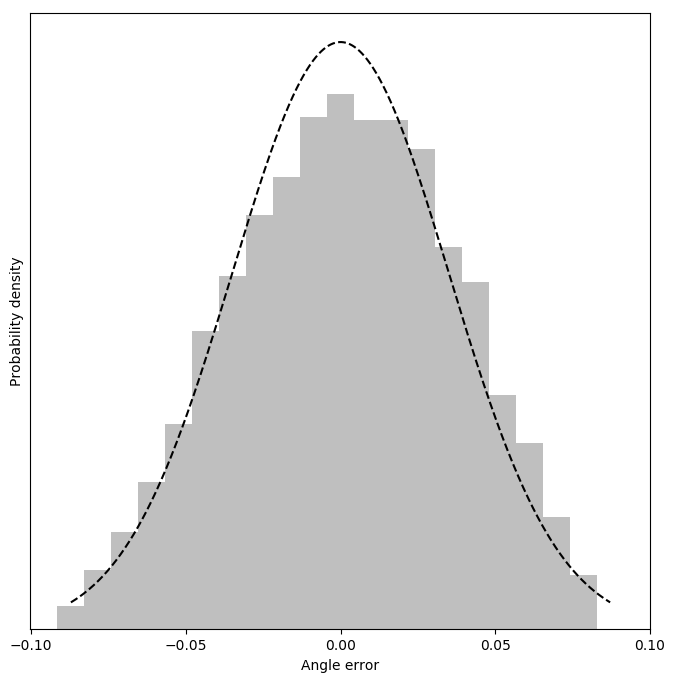
\includegraphics[width=\linewidth]{uncertainty}
  \end{minipage}
  \begin{minipage}{.5\textwidth}
    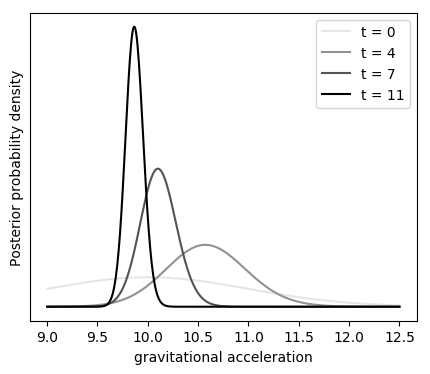
\includegraphics[width=0.97\linewidth]{posteriors}
  \end{minipage}
  \caption{Left: numerical forward propagation of time uncertainties through the pendulum model. Dashed line is the density function of the Gaussian used to model the uncertainty in our probabilistic model. Right: Sequence of posterior densities after observing $t=0, 3, 6, 9$ data points from light to dark, the lightest and darkest being respectively the prior and full posterior density. We see how the sequence of posteriors interpolate between the prior and full posterior distributions. }
  \label{uncertainty-posteriors}
\end{figure}



To model the pendulum problem in the Bayesian framework, we need to define a prior measure for the value of the parameter $g$ and find a distribution to model the measurements error.

To choose our prior measure, we first note that gravity attracts objects towards the center of the Earth. Given the coordinates system we have chosen, we know that the gravitational acceleration must be a positive value. We can also convince ourselves, by prior experiments or high-school knowledge, that the value of $g$ is close to $10$ and lower than $20$. Provided no additional information, the natural choice for the prior distribution to incorporate the knowledge stated above is to use a Gaussian distribution centered in $10$ with variance $1$, truncated to the interval $[0, 20]$.

For modelling the uncertainty in our measurements, we assume that measurement errors are symmetrical around $0$, and further assume an error in the measurements of approximately half a second. In order to obtain an approximation of the angle uncertainty, we propagate the time uncertainty through the forward response operator of the pendulum. This gives us an estimate of the uncertainty in the angle measurements. The forward propagation of the error is numerically estimated using the Monte Carlo method, described in Section 3, in which simulated time measurements were perturbated by a zero-mean Gaussian variable of standard deviation $0.5$ and used as new time measurements for the model. The result of this experiment leads us to model the uncertainty in the angles measurements with a zero-mean Gaussian of variance $0.035$. The left panel of Figure \ref{uncertainty-posteriors} illustrates the result of the numerical experiment.

We consider the estimation of the gravitational acceleration as a filtering problem, in which the sequence of likelihoods is defined using the construction proposed in equation (\ref{phi-seq})

\begin{equation}\label{pendulum-weights}
  \ell_t(x|g) := \exp\left(-\frac12\sum_{i=1}^t\left|x_i - \G_i(g)\right|^2\right),
\end{equation}

where $\G_i(g)$ is the solution of the equation (\ref{pendulum-ode}) at time $t = t_i$ with parameter $g$. The un-normalized posteriors resulting from this model are illustrated in the right panel of Figure \ref{uncertainty-posteriors}.

While the choice of prior is trivially light-tailed, we still need the following lemma to show that the pendulum problem is well-posed.

\begin{lemma} The pendulum problem satisfies Assumption \ref{assumption-fw}.
\end{lemma}

\begin{proof}
  We first prove that the solution $x(t)$ of the initial value problem is bounded, which is a stronger result than Assumption \ref{assumption-fw}(1). Let $g \in [0, 20]$ be fixed, we start by defining the Hamiltonian
  \begin{equation*}
    H(x, x') = \frac12 x'^2 - \frac{g}{l}\cos(x).
  \end{equation*}
  By simple calculations, one can show that $H$ is constant along the solution of the initial value problem. Since the initial values are $x_0 \in (0, \pi/2)$ and $x_0' = 0$, we have $H(x(t), x'(t)) = -\frac{g}{l}\cos(x_0) \in (-\frac{g}{l}, 0)$ for all $t > 0$. Assuming that $x(t)$ is not bounded, since $x$ is continuous and $x_0 \le \pi/2$, there is a time $t^*$ such that $x(t^*) = \pi$, giving
  \begin{equation*}
    H(x(t^*), x'(t^*)) = \frac12 x'(t^*)^2 - \frac{g}{l}\cos(x(t^*)) \ge -\frac{g}{l}\cos(\pi) = \frac{g}{l} > 0.
  \end{equation*}
  This contradicts $H(x(t), x'(t)) = H(x_0, x'_0) \in (-\frac{g}{l}, 0)$. Thus the solution of the initial value problem is bounded for every $g \in [0, 20]$ and $t > 0$ implying $\mathcal{G}_t$ is bounded as well, which in turn implies Assumption \ref{assumption-fw}(1).
  Furthermore, we know that the solution of the initial value problem is continuously differentiable with respect to $g$, it is thus locally Lipschitz continuous everywhere, and so is $\mathcal{G}$, thus completing the proof.
\end{proof}

We have proven that the pendulum problem is well posed, and can now use the Bayesian solution to the inverse problem to estimate the true value of $g$ from our measurements of the system. The next section will study numerical approximation methods to estimate this solution.

%%% Local Variables:
%%% mode: latex
%%% TeX-master: "Thesis"
%%% End:

\section{Proofs}

\subsection{bayes' rule}

\begin{theorem}
  \label{duley}
  Let $\mu, \nu$ be probability measures on $S \times T$, where $(S, \mathcal{A})$ and $(T, \mathcal{B})$ are measurable spaces. Let $(x, y) \in S \times T$. Assume that $\mu \ll \nu$ and that $\mu$ has Radon-Nikodym derivative $\phi$ with respect to $\mu$. Assume further that the conditional distributions of $x|y$ under $\nu$, denoted by $\nu^y(\text{d}x)$, exists. Then the conditional distribution of $x|y$ under $\mu$, denoted $\mu^y(\text{d}x)$, exists and $\mu^y(\text{d}x) \ll \nu^y(\text{d}x)$. The Radon-Nikodym derivative is given by

  \begin{equation}
    \frac{\text{d}\nu^y}{\text{d}\mu^y}(x) =  \begin{cases}
      \frac1{c(y)}\phi(x,y) & \text{if $c(y) > 0$, and}\\
      1 & \text{else,}
    \end{cases}  
  \end{equation}

  where $c(y) = \int_{S}\phi(x,y)\text{d}\mu^y(x)$ for all $y \in T$.
\end{theorem}

\begin{proof}
  See \cite{dudley_2002}.
\end{proof}

\begin{theorem}[Generalized Bayes' Rule]
  Assume that $\mathcal{G} : \Theta \rightarrow Y$ is continuous, that $\eta$ has a density $\rho$ with support equal to $Y$ and that $\mu_0(\Theta) = 1$. Then $\theta | y$ is distributed according to the measure $\mu^y$, with $\mu^y \ll \mu_0$ and Radon-Nikodym derivative with respect to $\mu_0$ given by

  \begin{equation}
    \frac{\text{d}\mu^y}{\text{d}\mu_0}(\theta) = \frac1{Z_y}\rho(y - \mathcal{G}(\theta)),
  \end{equation}

  where $Z_y$ is a constant that only dependends on $y$ and not on $\theta$, called the \textit{model evidence}.
\end{theorem}

\begin{proof}
  Let $\mathbb{Q}_0(\text{d}y) = \rho(y)\text{d}y$ and $\mathbb{Q}(dy|\theta) = \rho(y - \mathcal{G}(\theta))\text{d}y$. Since both measures have a Radon-Nikodym derivative with respect to the Lebesgue measure, we have

  \begin{equation*}
    \frac{\text{d}\mathbb{Q}}{\text{d}\mathbb{Q}_0}(y|\theta) = \frac{\text{d}\mathbb{Q}}{\text{d}\lambda}(y|\theta)\left(\frac{\text{d}\mathbb{Q}_0}{\text{d}\lambda}(y)\right)^{-1} = \frac{\rho(y - \mathcal{G}(\theta)}{\rho(y)} =: C(y)\rho(u - \mathcal{G}(\theta)).
  \end{equation*}

  Further define two measures $\nu_0, \nu$ on $Y \times \Theta$ by
  \begin{equation*}
    \begin{aligned}
      \nu_0(\text{d}y, \text{d}\theta) &= \mathbb{Q}_0(\text{d}y) \otimes \mu_0(\text{d}\theta)\\
      \nu(\text{d}y, \text{d}\theta) &= \mathbb{Q}(\text{d}y|\theta) \mu_0(\text{d}\theta).
    \end{aligned}
  \end{equation*}

  \note{not sure why $\mu(\Theta) = 1$ is required}
  
  Since $\mathcal{G}$ is continuous and $\mu(\Theta) = 1$, it is also $\mu_0$-measurable. Thus, $\nu$ is well-defined and continuous with respect to $\nu_0$ with Radon-Nikodym derivative

  \begin{equation*}
    \frac{\text{d}\nu}{\text{d}\nu_0}(y, \theta) = C(y)\rho(y - \mathcal{G}(\theta)).
  \end{equation*}

  Since $\nu_0$ is a product measure over $Y \times \Theta$, the random variables $y$ and $\theta$ are independent giving $\theta|y = \theta$. This implies that the conditional distribution of $\theta|y$ under $\nu_0$ is then $\nu_0^y = \mu_0$. In addition, since $\rho > 0$ we have $C(y) > 0$ and $\rho(y - \mathcal{G}(\theta)) > 0$ giving

  \begin{equation*}
    c(y) := \int_\Theta C(y)\rho(y - \mathcal{G}(\theta))\mu_0(\text{d}\theta) > 0 
  \end{equation*}

  Thus, by Theorem \ref{duley}, the conditional distribution of $\theta|y$ under $\nu$, denoted $\mu^y$, exists and its Radon-Nikodym derivative with respect to $\nu_0^y = \mu_0$ is

  \begin{equation*}
    \frac{\text{d}\mu^y}{\text{d}\mu_0}(\theta) = \frac1{c(y)}C(y)\rho(y - \mathcal{G}(\theta)) =  \frac1{Z_y}\rho(y - \mathcal{G}(\theta)).
  \end{equation*}
  
  where $Z_y = \int_\Theta\rho(y - \mathcal{G}(\theta))\mu_0(\text{d}\theta)$.
\end{proof}

\subsection{well-posedness}

\begin{assumption}\label{assumption-ll}
  The function $\Phi : \Theta \times Y \rightarrow \mathbb{R}$ has the following properties.
  
  \begin{enumerate}[i)]
  \item For every $\epsilon > 0$ and $r > 0$ there is an $M \in \mathbb{R}$ such that, for all $\theta \in \Theta$ and all $y \in Y$ with $\norm{y}_Y < r$,
    \begin{equation*}
      \Phi(\theta; y) \ge M - \epsilon\norm{\theta}_\Theta^2.
    \end{equation*}
  \item For every $r > 0$ there is a $K > 0$ such that, for all $\theta \in \Theta$ and $y \in Y$ with $\text{max}\{\norm{\theta}_\Theta, \norm{y}_Y\} < r$,
    \begin{equation*}
      \Phi(\theta; y) \le K.
    \end{equation*}

  \item For every $r > 0$ there is a $L > 0$ such that, for all $\theta_1, \theta_2 \in \Theta$ and $y \in Y$ with $\text{max}\{\norm{\theta_1}_\Theta, \norm{\theta_2}_\Theta, \norm{y}_Y\} < r$,

    \begin{equation*}
      |\Phi(\theta_1; y) - \Phi(\theta_2; y)| \le L\norm{\theta_1 - \theta_2}_\Theta.
    \end{equation*}

  \item For every $\epsilon > 0$ and $r > 0$ there is a $C \in \mathbb{R}$ such that, for all $y_1, y_2 \in Y$ with $\text{max}\{\norm{y_1}_Y, \norm{y_2}_Y\} < r$, and for all $\theta \in \Theta$,

    \begin{equation*}
      |\Phi(\theta; y_1) - \Phi(\theta; y_2)| \le \exp(\epsilon\norm{\theta}_\Theta^2 + C)\norm{y_1 - y_2}_Y.
    \end{equation*}
  \end{enumerate}
\end{assumption}

\begin{assumption}\label{assumption-fw}
  The function $\mathcal{G} : \Theta \rightarrow \mathbb{R}^N$ satisfies the following.

  \begin{enumerate}[i)]
  \item For every $\epsilon > 0$ there is an $M \in \mathbb{R}$ such that for all $\theta \in \Theta$,
    \begin{equation*}
      |\mathcal{G}(\theta)|_\Gamma \le \exp(\epsilon \norm{\theta}_\Theta^2 + M).
    \end{equation*}
  \item For every $r > 0$ there is a $K > 0$ such that, for all $\theta_1, \theta_2 \in \Theta$ with $\text{max}\{\norm{\theta_1}_\Theta, \norm{\theta_2}_\Theta\} < r$,
    \begin{equation*}
      |\mathcal{G}(\theta_1) - \mathcal{G}(\theta_2)|_\Gamma \le K\norm{\theta_1 - \theta_2}_\Theta.
    \end{equation*}
  \end{enumerate}
\end{assumption}

\begin{lemma} \label{fw-implies-ll}
  Assume that $\mathcal{G} : \Theta \rightarrow \mathbb{R}^N$ satisfies Assumption \ref{assumption-fw}. Then, for any covariance matrix $\Gamma$ and the potential function $\Phi : \Theta \times \mathbb{R}^N \rightarrow \mathbb{R}$ given by
  \begin{equation*}
    \Phi(\theta; y) = \frac12 \left|\Gamma^{-1/2}(y - \mathcal{G}(\theta))\right|^2 = \frac12 \left|y - \mathcal{G}(\theta)\right|^2_\Gamma
  \end{equation*}

  satisfies Assumption \ref{assumption-ll} with $(Y, \norm{\cdot}_Y) = (\mathbb{R}^N, \norm{\cdot}_\Gamma)$.
\end{lemma}

\begin{proof} This is trivial, can I skip this proof?
\end{proof}

\begin{lemma} The pendulum problem satisfies Assumption \ref{assumption-ll}.
\end{lemma}

\begin{proof}
  We first prove that the solution $x(t)$ of the initial value problem is bounded, which is a stronger property than property i). We start by defining the Hamiltonian
  \begin{equation*}
    H(x, x') = \frac12 x'^2 - \frac{g}{l}\cos(x).
  \end{equation*}
  By simple calculation, one can show that $H$ is constant along the solution of the initial value problem. Since the initial values are $x_0 \in (0, \pi/2)$ and $x_0' = 0$, we have $H(x(t), x'(t)) = -\frac{g}{l}\cos(x_0) \in (-\frac{g}{l}, 0)$ for all $t > 0$. Assuming that $x(t)$ is not bounded, since $x$ is continuous and $x_0 \le \pi/2$, there is a time $t^\star$ such that $x(t^\star) = \pi$, giving
  \begin{equation*}
    H(x(t^\star), x'(t^\star)) = \frac12 x'(t^\star)^2 - \frac{g}{l}cos(x(t^\star)) \ge -\frac{g}{l}\cos(\pi) = \frac{g}{l} > 0.
  \end{equation*}
  This contradicts $H(x(t), x'(t)) = H(x_0, x'_0) \in (\frac{g}{l}, 0)$.Thus the solution of the initial value problem is bounded and so is $\mathcal{G}$, proving i).
  Furthermore, we know that the solution of the initial value problem is continuously differentiable with respect to $g$, it is thus locally Lipschitz continuous everywhere, and so is $\mathcal{G}$, thus completing the proof.
\end{proof}

\subsection{smc convergence}

\begin{lemma}
  Let $P(E)$ denote the set of all probability measures on $E$. For every $\mu$ and $\nu$ random variables with values in $P(E)$, we define

  \begin{equation*}
    d(\mu, \nu) := \underset{f}{\text{sup}} \sqrt{\expec{|\mu f - \nu f|^2}},
  \end{equation*}

  where the supremum is taken over all $f : E \rightarrow \mathbb{R}$ with $|f|_\infty \le 1$, and $\mu f$ denotes the integral of $f$ under $\mu$. Then $d$ is a metric over the space of random measures over $E$.
\end{lemma}

\begin{proof} Trivial enough to skip the proof?
\end{proof}

\begin{definition}
  Let $M \in \mathbb{N}$, for every $\mu \in P(E)$ we define $S^M\mu$ by

  \begin{equation*}
    S^M\mu = \frac1{M}\sum_{i=1}^M\delta_{u_i},
  \end{equation*}

  where $u^{(1)}, \ldots, u^{(M)}$ are i.i.d. random variables distributed according to $\mu$. From the randomness of the samples $u^{(1)}, \ldots, u^{(M)}$, it follows that $S^M\mu$ is a random variable with values in $P(E)$. The operator $\mu \mapsto S^M\mu$ is called \textit{sampling operator}.
\end{definition}

\begin{lemma}\label{sampling-bound}
  The sampling operator satisfies

  \begin{equation*}
    \underset{\mu \in P}{\text{sup}}\ d(S^M\mu, \mu) \le \frac1{\sqrt{M}}
  \end{equation*}
\end{lemma}

\begin{proof}
  Let $\mu$ be an element of $P(E)$ and $u^{(1)}, \ldots, u^{(M)}$ be i.i.d. random variables distributed according to $\mu$. For every $f$ with $|f|_\infty \le 1$ we have 
  
  \begin{equation*}
    (S^M\mu)f - \mu f = \frac1{M}\sum_{i=1}^Mf(u^{(i)}) - \mu f = \frac1{M}\sum_{i=1}^Mf_i,
  \end{equation*}

  where $f_i = f(u^{(i)}) - \mu f$. This gives

  \begin{equation*}
    \left|(S^M\mu - \mu)f\right|^2
    = \left(\frac1{M}\sum_{i=1}^Mf_i\right)^2
    = \frac1{M^2}\sum_{i,j=1}^Mf_if_j.
  \end{equation*}

  Since we are interested in the expected value of this term, we now consider $\expec{f_if_j}$. For $i \neq j$, $f_i$ and $f_j$ are independent random variables, thus $\expec{f_if_j} = \expec{f_i}\expec{f_j}$, and since $u^{(i)} \sim \mu$, we have $\expec{f_i} = \expec{f(u^{(i)})} - \mu f = 0$, giving $\expec{f_if_j} = 0$ for $i \neq j$. Furthermore, since $|f|_\infty \le 1$ we have

  \begin{equation*}
    \expec{f_i^2} = \text{Var}[f(u^{(i)})] = \expec{f(u^{(i)})^2} - \expec{f(u^{(i)})}^2 \leq 1.
  \end{equation*}

  By linearity of the expected value, we then have for every $f$ with $|f|_\infty \le 1$

  \begin{equation*}
    \expec{\left|(S^M\mu)f - \mu f\right|^2} = \frac1{M^2}\sum_{i=1}^M\expec{f_i^2} \le \frac1{M}.
  \end{equation*}

  Taking the square root on both sides of the equation and the supremum over all such $f$ yields the desired result.
\end{proof}

\begin{assumption}\label{kappa-assumption}
  There exists a $\kappa > 0$ such that for every $n \in \mathbb{N}$ and $\theta \in \Theta$

  \begin{equation*}
    \kappa \leq l_n(\theta) \leq 1/\kappa.
  \end{equation*}

  This assumption is weaker than \note{assumption 2.6 in Stuart 2010} if $\Theta$ is compact.
\end{assumption}

\note{$\Phi_n$ is defined in Beskos 2015, as $\Phi_n = K_nL_{n-1}$ where $K_n$ is a transition kernel and $L_{n-1}$ is the Bayes' rule update, meaning $(L_{n-1}\mu)(du) = \frac{l_{n-1}(u)}{\mu(l_{n-1})}\mu(du)$, where $l_i$ are the likelihoods of the sequence. These values will be properly defined in the thesis and another notation will probably be used. }
\begin{lemma} \label{seq-bound}
  Assume that the likelihoods $l_i$ satisfy Assumption \ref{kappa-assumption}. Then for any $n \in \mathbb{N}$ and $\mu, \nu \in P(E)$,

  \begin{equation*}
    d(\Phi_n\mu, \Phi_n\nu) \leq \frac2{\kappa^2}d(\mu, \nu).
  \end{equation*}
\end{lemma}

\begin{proof}
  Let $f : E \rightarrow \mathbb{R}$ be a measurable function with $|f|_\infty \le 1$, we then have

  \begin{equation*}
    \begin{aligned}
      (\Phi_n\mu - \Phi_n\nu)f
      &= (K_nL_{n-1}\mu - K_nL_{n-1}\nu)f \\
      &= \frac{\mu(l_{n-1}K_n(f))}{\mu(l_{n-1})} - \frac{\nu(l_{n-1}K_n(f))}{\nu(l_{n-1})} \\
      &= \frac{\mu - \nu}{\mu(l_{n-1})}(l_{n-1}K_n(f)) + \frac{\nu(l_{n-1}K_n(f))}{\mu(l_{n-1})} - \frac{\nu(l_{n-1}K_n(f))}{\nu(l_{n-1})}\\
      &= \frac{\mu - \nu}{\mu(l_{n-1})}(l_{n-1}K_n(f)) + \nu(l_{n-1}K_n(f))\left(\frac1{\mu(l_{n-1})} - \frac1{\nu(l_{n-1})}\right)\\
      &= \frac{\mu - \nu}{\mu(l_{n-1})}(l_{n-1}K_n(f)) + \frac{ \nu(l_{n-1}K_n(f))}{\mu(l_{n-1})\nu(l_{n-1})}(\nu - \mu)(\l_{n-1}).
    \end{aligned}
  \end{equation*}
  
  By Minkowski's inequality, we then have

  \begin{equation*}
    \begin{aligned}
      \sqrt{\expec{|(\Phi_n\mu - \Phi_n\nu)f|^2}}
      &\leq \expec{\left|\frac{\mu - \nu}{\mu(l_{n-1})}(l_{n-1}K_n(f))\right|^2}^{\frac12}\\
      &+ \expec{\left|\frac{ \nu(l_{n-1}K_n(f))}{\mu(l_{n-1})\nu(l_{n-1})}(\nu - \mu)(\l_{n-1})\right|^2}^{\frac12}      .
    \end{aligned}
  \end{equation*}


  In the second term, we observe that $\frac{\nu(l_{n-1}K_n(f))}{\nu{l_{n-1}}}$ is the expectation of $f$ under the probability measure $\Phi_n \nu$. Together with $|f|_\infty \le 1$, this gives us $\frac{\nu(l_{n-1}K_n(f))}{\nu{l_{n-1}}} \le 1$. Similarly, since $l_{n-1}(u) \ge 1/\kappa$ for all $u$, it holds that $\mu(l_{n-1}) \ge \kappa$ and $1 / \mu(l_{n-1}) \le 1/\kappa$. From these two bounds, we obtain

  \begin{equation*}
    \begin{aligned}
      \sqrt{\expec{|(\Phi_n\mu - \Phi_n\nu)f|^2}}
      &\le \frac1\kappa\expec{|(\mu - \nu)(l_{n-1}K_n(f))|^2}^{\frac12}\\
      &+ \frac1\kappa\expec{|(\mu - \nu)(l_{n-1})|^2}^{\frac12}.
    \end{aligned}
  \end{equation*}


  Finally, using that $0 \le l_{n-1} \le 1/\kappa$, we have $|\kappa l_{n-1}|_\infty \le 1$ and similarly $[l_{n-1}K_n(f)](u) = \int_{\Theta} f(y)l_{n-1}(u)K_n(u, \text{d}y) \leq |fl_{n-1}|_\infty K_n(\Theta, u) \leq 1 / \kappa$, thus making $|\kappa l_{n-1}K_n(f)|_\infty \leq 1$. We can thus bound our expression by the supremum over all $g$ with $|g|_\infty \le 1$ and get

  \begin{equation*}
    \sqrt{\expec{|(\Phi_n\mu - \Phi_n\nu)f|^2}} \le \frac2{\kappa^2}\underset{g}{\text{sup}} \sqrt{\expec{|\mu g - \nu g|^2}} =  \frac2{\kappa^2}d(\mu, \nu).
  \end{equation*}

  Since this result is valid for all $f$ with $|f|_\infty \le 1$, taking the supremum on the left side yields the desired result.
\end{proof}

\note{$\nu_n^M = S^M\Phi_n\nu_{n-1}^M$ and for $n=0$ we dirac approximate with an initial sample of $\nu_0$, this will be better defined in the presentation of the algorithm.}
\begin{theorem}
  Assume that the likelihoods $l_i$ satisfy Assumption \ref{kappa-assumption} and consider the SMC algorithm with $M_{thresh} = M$. Then, for any $n \in \mathbb{N}$,

  \begin{equation*}
    d(\nu_n, \nu_n^M) \leq \sum_{j=0}^n\left(\frac2{\kappa^2}\right)^j\frac1{\sqrt{M}}.
  \end{equation*}
\end{theorem}

\begin{proof}
  For $n=0$, the result hold by direct application of Lemma \ref{sampling-bound}. For $n > 0$ we have by the triangle inequality and Lemmata \ref{sampling-bound} and \ref{seq-bound}

  \begin{equation*}
    \begin{aligned}
      d(\nu_n, \nu_n^M)
      &= d(\Phi_n\nu_{n-1}, S^M\Phi_n\nu_{n-1}^M)\\
      &\le d(\Phi_n\nu_{n-1}, \Phi_n\nu_{n-1}^M) + d(\Phi_n\nu_{n-1}^M, S^M\Phi_n\nu_{n-1}^M)\\
      &\le \frac2{\kappa^2}d(\nu_{n-1}, \nu_{n-1}^M) + \frac1{\sqrt{M}}.
    \end{aligned}
  \end{equation*}

  Iterating on $n$ gives the desired result.
\end{proof}

%%% Local Variables:
%%% mode: latex
%%% TeX-master: "Thesis"
%%% End:

\section{Numerical solution to the pendulum problem}
In this section, we present and analyse the numerical solution of the filtering problem associated to the pendulum experiment. We then run the SIS and SMC algorithms to approximate the expected value of the full posterior distribution and analyze their empirical convergence properties. As a reference, we also present the result of the MCMC approximation to the complete data set.

In the first experiment, we estimate the solution to the Bayesian inverse problem found by considering all the available data collected during the physical experiment. We use the MCMC algorithm for $10,000$ steps after a burn-in period of $500$ steps and construct the Markov chain using Metropolis-Hasting kernel with Gaussian proposals of variance $0.1$. The burn-in period runs the Markov Chain for $500$ steps without collecting the generated samples needed to reach the region of high probability. After $5$ runs of the algorithm, we find an mean estimate of $\expec{u|y} = 9.86 \pm \mathcal{O}(10^{-3})$ and a variance of $\mathcal{O}(10^{-6})$. This result is consistent with the unnormalized likelihoods presented in Figure \ref{uncertainty-posteriors}, and validate the theoretical results stated in Lemma \ref{sampling-bound}. A typical run of the algorithm is given in Figure \ref{mcmc-figure}.

\begin{figure}[!b]
  \label{mcmc-figure}
  \begin{minipage}{.43\textwidth}
    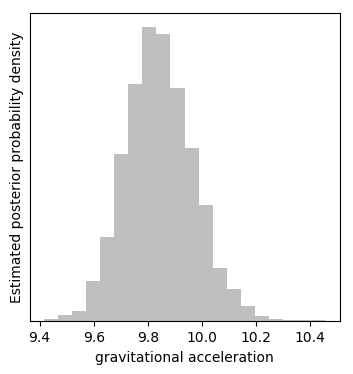
\includegraphics[width=\linewidth]{mcmc}
  \end{minipage}
  \begin{minipage}{.5\textwidth}
    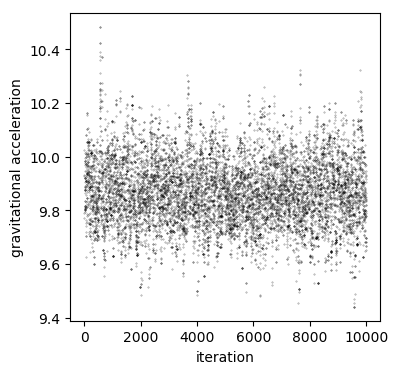
\includegraphics[width=0.97\linewidth]{mcmc-mixin}
  \end{minipage}
  \caption{Left: estimated posterior distribution using $M=10,000$ samples from the MCMC algorithm with burn-in period of $500$ samples. Right: samples of the Markov chain for one run on the MCMC algorithm. We see that the burn-in period allows to have all actualy samples in the zone of high density and converge.}
\end{figure}

\begin{figure}[htbp]
  \begin{minipage}{.5\textwidth}
    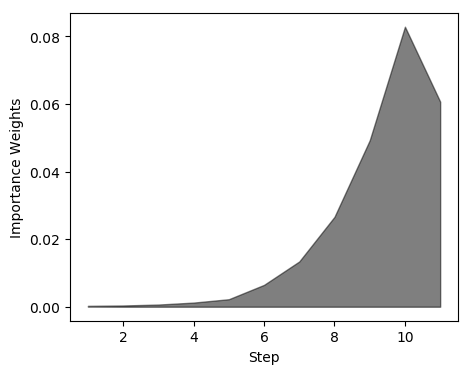
\includegraphics[width=\linewidth]{importance-weights-sis}
  \end{minipage}
  \begin{minipage}{.5\textwidth}
    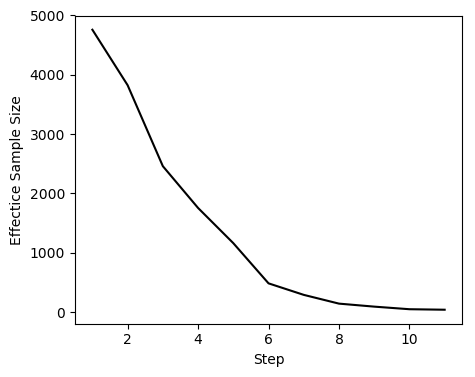
\includegraphics[width=0.97\linewidth]{ess-decay}
  \end{minipage}
  \caption{Left: the evolution of the importance weights of the particle estiamtes. The upper and lower bounds of the shaded area represent the value of the largest and smaller importance weight of the population. We can see that close to the end, a single particle contain almost all mass of the estimated probability measure. Right: evolution of the ESS over time, we see that after half the total number of iterations, the ESS is already only almost 1.}\label{sis-figure}

  \bigskip
  
  \begin{minipage}{.5\textwidth}
    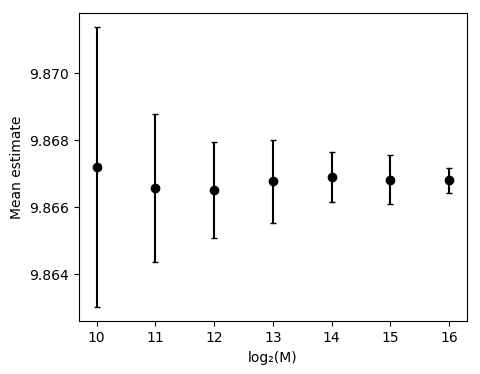
\includegraphics[width=\linewidth]{mean-estimate}
  \end{minipage}
  \begin{minipage}{.5\textwidth}
    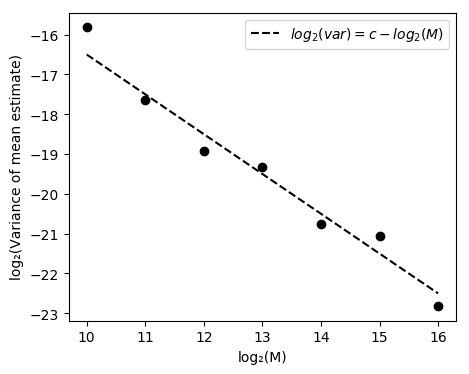
\includegraphics[width=0.97\linewidth]{var-of-estimate}
  \end{minipage}
  \caption{Both plots consider $40$ runs of $M$-particles SMC estimates of the posterior expected value. Left: Each point is the mean and variance over the $40$ SMC runs for each $M$. Right: Logarithmic plot of the variance of $40$ estimates. Line illustrates the asymptotical $\mathcal{O}(M^{-1})$ behaviour of the variance proved in Theorem \ref{smc-convergence}. }\label{smc-figure}
\end{figure}


However, we are interested in approximating the sequence of filtering posterior distributions arising from the pendulum problem where the data only becomes available one observation at a time. In the following experiments, we use the sequence of importance weights given in (\ref{pendulum-weights}). Since we fulfill all assumptions stated in Lemma \ref{easy-lemma}, it also satisfies Assumption \ref{kappa-assumption} and the solution provided by the SIS and SMC algorithms weakly converge in $M$ to the true posteriors. In both algorithms, we use Metropolis-Hastings kernels with Gaussian proposals of variance $0.05$. 

In the second experiment, we illustrate why the step of resampling is crucial in the SMC algorithm. We run the SIS algorithm with $M=5,000$ particles and monitor the ESS as well as the importance weights over time. As expected, the experiment shows that the variance of the weights increases with both very large and very small weights, meaning that most of the probability mass of the particle estimate is contained in only a few estimate. Monitoring the ESS confirms this is also shown by the convergence of the ESS to $1$. This makes the variance These two results are shown in Figure \ref{sis-figure}.

In a last experiment, we run the SMC algorithm with $M_{thresh} = M/2$ for several values of $M$ and repeat the experiment $40$ times per configuration. We use $5$ MCMC updates for the correction step to improve the approximations, this claim is theoretically justified by \cite{marion2018finite}. Figure \ref{smc-figure} reports the result of the experiment, showing the convergence of the posterior expected value estimate.

To conclude this section, we compare computational costs of the MCMC and SMC algorithms. Each time new data becomes available, the MCMC algorithm needs to sequentially re-sample $M$ values from the associated Markov chain. This in turn leads to $M$ evaluations of the likelihood function, requiring to numerically solve $M$ initial value problems. While the SMC algorithm also needs to perform $M$ evaluations of the likelihood function to update the particles, since each particle is independent these evaluations do not need to be made sequentially. This allows to parallelize the evaluation of the likelihood function and potentially strongly reduce the cost of updating an existing estimate as shown by \cite{lee2010utility}.

%%% Local Variables:
%%% mode: latex
%%% TeX-master: "Thesis"
%%% End:

\section{Conclusion}

We have presented inverse problems and filtering problems for cases where more data becomes available over time. We have shown how the Bayesian framework provides a well-posed solution to the inverse problem and how Bayesian filtering gives a natural and sound formalism to incorporate new data to the existing knowledge about the unknown parameters. We have then shown how common numerical estimation algorithms fail at efficiently approximating the sequence of filtering posterior distributions and have constructed the SMC algorithm to provide an estimator that is not only asymptotically correct, but also solves many practical difficulties encountered when running the algorithm with finitely many particles available for approximation.

However, many areas could be explored to extend this work. Firstly, we have used a very simple model of the pemdulum. We could define a new model to take into account air friction an treat the friction coefficient of the pendulum's mass as an additional parameter of the model. Since the pendulum was let go by a human operator in the experiments, there is also uncertainty in the initial angle of the pendulum which could be taken into account in the model. These additional modeling choice could not only improve the quality of our estimate, but would also be of interest to test the SMC algorithm on higher-dimensional models with latent variables. Secondly, we did not go in great details about the choice on Markov kernels for the MCMC, SIS and SMC algorithms. While Metropolis-Hastings kernels are a very common choice, contructing such Markov chains has been a very active research area from which it could be possible to use more recent results. Also, the use of Markov kernels was only justified by empirical observations, and we have not given any theoretical proof of the impact of these kernels on the convergence properties of the algorithms.

%%% Local Variables:
%%% mode: latex
%%% TeX-master: "Thesis"
%%% End:


\listoffigures

\newpage

\bibliographystyle{alpha}
\bibliography{Bibliography}

\end{document}
%%% Local Variables:
%%% mode: latex
%%% TeX-master: t
%%% End:
